\documentclass{article}%
\usepackage[T1]{fontenc}%
\usepackage[utf8]{inputenc}%
\usepackage{lmodern}%
\usepackage{textcomp}%
\usepackage{lastpage}%
\usepackage[head=40pt,margin=0.5in,bottom=0.6in]{geometry}%
\usepackage{graphicx}%
%
\title{\textbf{Curcio: la expansión monetaria no causa la hiperinflación}}%
\author{Diario El Universal}%
\date{02/12/2018}%
%
\begin{document}%
\normalsize%
\maketitle%
\textbf{URL: }%
http://www.eluniversal.com/economia/27222/curcio{-}la{-}expansion{-}monetaria{-}no{-}causa{-}la{-}hiperinflacion\newline%
%
\textbf{Periodico: }%
EU, %
ID: %
27222, %
Seccion: %
economia\newline%
%
\textbf{Palabras Claves: }%
NO\_TIENE\newline%
%
\textbf{Derecho: }%
CONTEXTO, %
Otros Derechos: %
, %
Sub Derechos: %
\newline%
%
\textbf{EP: }%
NO\newline%
\newline%
%
\textbf{\textit{“En los últimos 90 días el índice de monetización disminuyó en 62\%”}}%
\newline%
\newline%
%
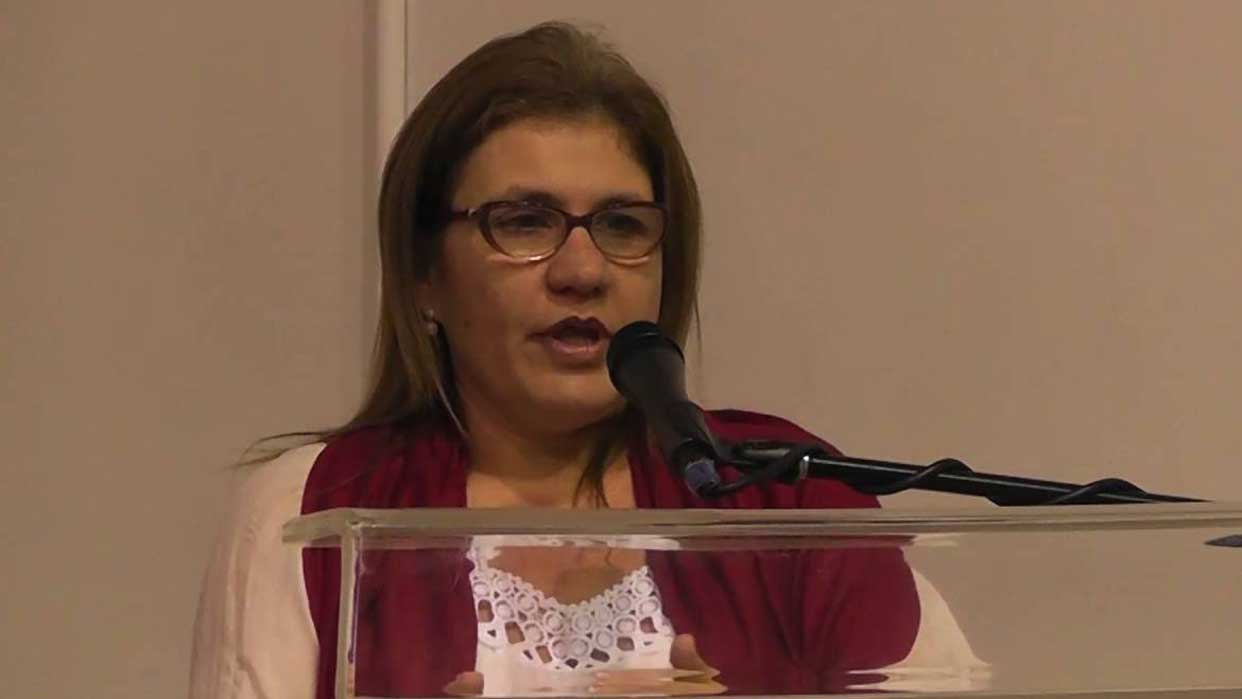
\includegraphics[width=300px]{67.jpg}%
\newline%
%
Caracas.{-}~Pascualina Curcio, economista y profesora titular de la Universidad Simón Bolívar (USB), considera  que para lograr destrancar el juego económico son necesarias las siguientes acciones: recuperar la producción petrolera; fortalecer el bolívar a través de su anclaje directo en el oro y el petróleo; recuperar las reservas internacionales mediante controles estrictos del uso de las divisas y el incremento de la cantidad de oro en el BCV; avanzar en la construcción de otra economía en la que los ingresos por exportación de petróleo queden en Venezuela y tributen para la producción interna, a través de la socialización, distribución de la producción y el fortalecimiento de la economía estadal y comunal, lo cual resulta relativamente más viable cuando el 98\% de los ingresos del país son propiedad del Estado y por tanto de los venezolanos.%
\newline%
%
MARBELYS MAVÁREZ LAGUNA%
\newline%
%
Hiperinflación y su causa%
\newline%
%
Uno de los principales objetivos que debe alcanzar el Gobierno, de acuerdo con Curcio, consiste en “derrotar el ataque a la moneda que es la causa originaria y determinante de la hiperinflación. Esto afecta a todos sin discriminación y tiene un doble efecto. Por una parte, pulveriza el salario y por la otra contrae los niveles de producción. Han manipulado políticamente el tipo de cambio de 8,96 Bs.F/\$ a 40 millones Bs.F/\$”.%
\newline%
%
Desde su punto de vista, no es cierto que la expansión monetaria sea la causa de la hiperinflación. Por el contrario, en “estos 90 días, el índice de monetización (cantidad de dinero que circula con respecto al tamaño de la economía) ha disminuido 62\% y sin embargo hemos observado cómo siguen aumentando los precios. Desde el año 2013, dicho índice ha caído 91\% pasando de 66\% en 2013 a 6\% en 2018”.%
\newline%
%
De acuerdo con la economista “el ataque a la moneda y la hiperinflación que de ella se deriva explica el 40\% de la caída de la producción nacional, por lo tanto, cualquier esfuerzo de reactivación de los sectores productivos, incluso el petrolero, se ve contrarrestado por el efecto perverso de la manipulación del tipo de cambio y la hiperinflación”, sostuvo.%
\newline%
%
¡A recuperar las reservas!%
\newline%
%
“Es necesario recuperar las reservas internacionales, lo cual implica evitar la fuga de divisas que ingresan por exportación de petróleo, establecer controles estrictos en el uso de dichas divisas y no seguir transfiriéndolos a un sector privado que históricamente se ha apropiado de más de 700 mil millones de dólares, de los cuales más del 60\% están fuera de nuestras fronteras”, aseguró Curcio.%
\newline%
%
Manifestó que asignar divisas a tasa preferencial a los grandes capitales transnacionales, no solo no garantiza la recuperación de la producción, sino que se revierte en la medida en que impide que podamos aumentar nuestras reservas internacionales”, asegura, al tiempo que agrega: “aumentar las reservas también pasa por garantizar que el oro que es extraído de nuestras minas sea llevado a las bóvedas del Banco Central, sea certificado y monetizado.%
\newline%
%
Se refirió a las 2 toneladas mensuales de oro que son llevadas al BCV. “Estas, al monetizarlas, cuentan como reservas internacionales. A diferencia de cualquier país, nosotros no debemos entregar nuestros dólares o euros para comprar oro”, dijo la economista.%
\newline%
%
\end{document}